% Generated by AP Math GOLD PILOT deterministic Python generator.
% input id: 07_calculus_step_count
\documentclass{article}
\usepackage[margin=1cm]{geometry}
\def\pgfsysdriver{pgfsys-dvisvgm.def}
\usepackage{amssymb}
\usepackage{pgfplots}
\pgfplotsset{compat=1.18}
\pagestyle{empty}
\begin{document}
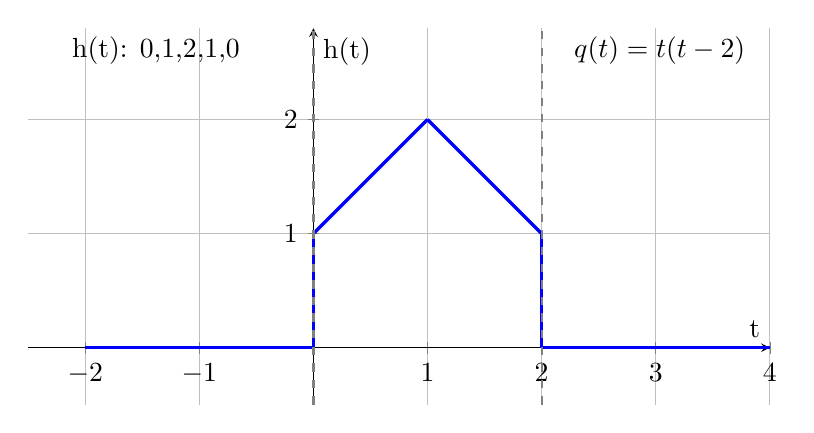
\begin{tikzpicture}
\begin{axis}[width=11cm,height=9cm,axis equal image,axis lines=middle,grid=major,xmin=-2.5,xmax=4,ymin=-0.5,ymax=2.8,xlabel={t},ylabel={h(t)},clip=true]
\draw[blue, solid, line width=1.2pt] (axis cs:-2,0) -- (axis cs:0,0);
\draw[blue, solid, line width=1.2pt] (axis cs:0,0) -- (axis cs:0,1);
\draw[blue, solid, line width=1.2pt] (axis cs:0,1) -- (axis cs:1,2);
\draw[blue, solid, line width=1.2pt] (axis cs:1,2) -- (axis cs:2,1);
\draw[blue, solid, line width=1.2pt] (axis cs:2,1) -- (axis cs:2,0);
\draw[blue, solid, line width=1.2pt] (axis cs:2,0) -- (axis cs:4,0);
\draw[gray, dashed, line width=0.8pt] (axis cs:0,-0.5) -- (axis cs:0,2.8);
\draw[gray, dashed, line width=0.8pt] (axis cs:2,-0.5) -- (axis cs:2,2.8);
\node[anchor=south west] at (axis cs:2.2,2.4) {$q(t)=t(t-2)$};
\node[anchor=south west] at (axis cs:-2.2,2.4) {h(t): 0,1,2,1,0};
\end{axis}
\end{tikzpicture}
\end{document}
